%----------- Capítulo 3: Especificação do Software -------------

\chapter{Especificação do Software}
O software em questão consiste em um serviço web que tem como principal funcionalidade responder a rota entre dois pontos informados com menor tempo de viagem utilizando o sistema de transporte público. 
Nas subseções a seguir serão apresentados os requisitos do sistema bem como sua arquitetura.

\section{Requisitos do Sistema}
O primeiro passo para o desenvolvimento de qualquer sistema computacional é levantar seus requisitos. A seguir estão listadas os requisitos do sistema.

\subsection{Requisitos Funcionais}
\begin{itemize}
	\item O software deverá retornar para o usuário a rota com menor tempo de viagem entre dois pontos informados.
	\item O software deverá mostrar a rota resultante desenhada em um mapa, diferenciando as linhas de transporte por cor, e também no formato texto como uma sequência de passos.
	\item O software deverá receber do usuário os pontos de partida/destino no formato de endereço e/ou marcando-os no mapa.
	\item O software deverá receber o horário de partida no formato HH:MM.
	\item O software deverá funcionar independente de qual fonte de dados for escolhida, contudo que esta respeite o padrão GTFS.
\end{itemize}

\subsection{Requisitos Não-Funcionais}
\begin{itemize}
	\item O software deverá ser disponibilizado como livre, possibilitando futuras contribuições.
	\item O software deverá ser disponibilizado no formato de um serviço web.
	\item O software devera utilizar o padrão GTFS para o arquivo fonte de dados contendo as rotas do sistema público de transporte de determinada cidade.
	\item O software deverá ser desenvolvido em linguagem Java e, para o núcleo web, javascript.
	\item O software deverá utilizar um banco de dados de grafos para armazenamento das rotas do sistema de transporte público.
\end{itemize}

\section{Arquitetura do Sistema}
O sistema em questão é composto de quatro núcleos principais: \emph{Core, GTFS Importer, Web Service} e um Cliente (o qual consiste num \emph{Cliente Web} atualmente). 
O projeto de fluxo padrão do sistema como um todo é mostrado na figura \ref{fig:arquitetura}.

\begin{figure}[!htb]
	\centering
	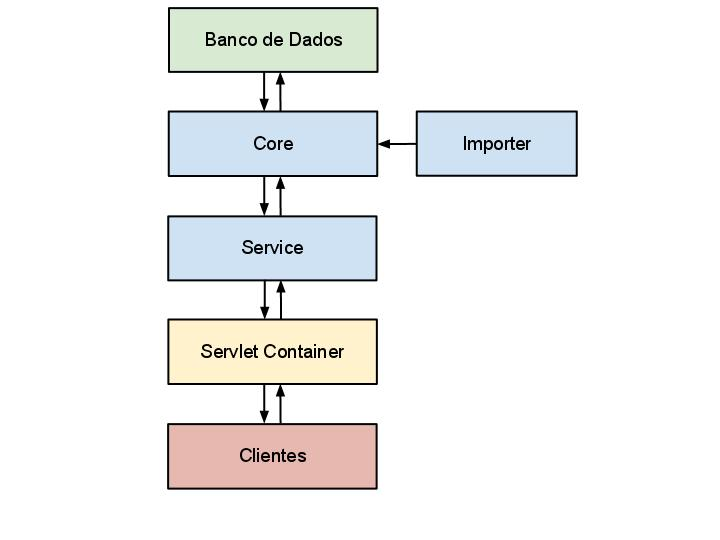
\includegraphics[width=0.6\textwidth]{./arquitetura.jpg}
	\caption[ImgArquitetura]{Visão geral da arquitetura do sistema.}
	\fonte{Autoria Própria}
	\label{fig:arquitetura}
\end{figure}

Primeiramente o usuário informa os pontos de origem e destino para o Cliente marcando-os no mapa disponibilizado ou fornecendo o endereço por extenso nas devidas caixas de texto, juntamente com o horário de partida no formato HH:MM. 
Feito isso, os dados coletados são enviados ao Web Service através de um HTTP POST. 
Este é responsável pela execução da query para encontrar a rota contendo o caminho mínimo, sendo o acesso ao banco de dados realizado através dos métodos e entidades contidos no \emph{Core}.
Ao terminar de executar a query no banco, o \emph{Web Service} responde ao Cliente as informações sobre a rota resultante através de um objeto serializado no formato JSON, sendo estas por fim mostradas para o usuário de duas formas: uma sequência de passos em formato texto e visualmente através do desenho da rota no mapa.

Para que qualquer consulta seja bem sucedida, é necessário que o banco de dados esteja populado com as informações do arquivos no padrão GTFS, população a qual é realizada através do núcleo \emph{GTFS Importer}.
A seguir uma explicação detalhada de cada módulo do sistema.

\subsection{Core}
Este módulo foi projetado para conter todas as representações das entidades que compõem o sistema, bem como suas respectivas \emph{factories} e um controle de acesso ao banco de dados.
O diagrama de projeto do pacote \emph{Core} é mostrado na \ref{fig:core}.

\begin{figure}[!htb]
	\centering
	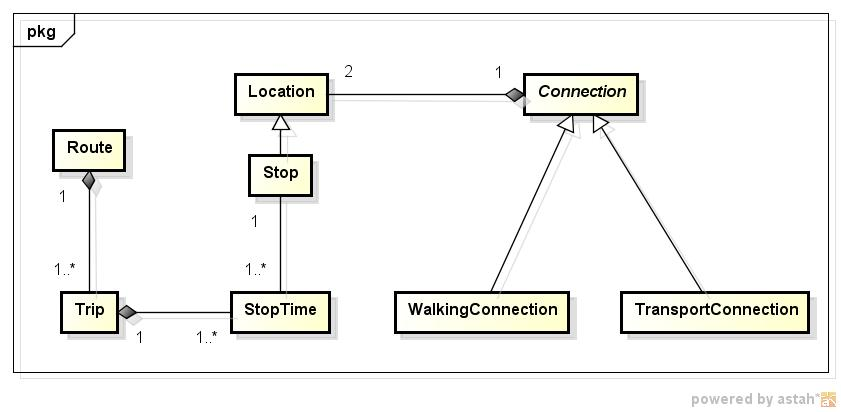
\includegraphics[width=1\textwidth]{./CoreDiagram.jpg}
	\caption[ImgCore]{Visão geral da arquitetura do Core.}
	\fonte{Autoria Própria}
	\label{fig:core}
\end{figure}

Como se pode observar, o \emph{Core} é composto pelas seguintes entidades advindas do padrão GTFS:

\begin{itemize}
	\item \textbf{Route}: contém informações a respeito de uma linha de transporte público, tais como o nome da rota, o meio de transporte utilizado, e as \emph{Trips} que a compõem.
	\item \textbf{Trip}: é uma sequência de duas ou mais \emph{StopTime}, ou seja, dois ou mais pontos de parada que ocorrem em um tempo determinado.
	\item \textbf{Location}: consiste em um ponto de coordenadas geográficas e suas respectivas conexões de entrada e saída com outros pontos.
	\item \textbf{Stop}: é uma \emph{Location} que consiste em um ponto de parada  de veículos para entrada e saída de passageiros.
	\item \textbf{StopTime}: contém informações de horários de partida e chegada de veículos em uma determinada \emph{Stop} pertencente a uma \emph{Trip}.
	\item \textbf{Connection}: é uma conexão entre dois pontos, podendo ser entre duas \emph{Stops} (\emph{TransporteConnection}) ou entre uma \emph{Stop} e uma \emph{Location} (\emph{WalkingConnection}).
	\item \textbf{Calendar}: especifica quando determinado serviço de transporte começa e termina, bem como os dias da semana nos quais o serviço está disponível.
\end{itemize}

Para a criação no sistema de cada uma destas entidades foi utilizado o conceito de \emph{factories}. 
Uma \emph{factory} nada mais é que um \emph{design pattern} que consiste em uma interface para a criação de famílias de objetos correlatos ou dependentes.
Desta forma, cada entidade do \emph{Core} possui sua respectiva \emph{factory} não somente para criação de objetos mas também para retornar todos os objetos de um determinado tipo de entidade.

Todos estes objetos são armazenados no banco de dados através da classe \emph{DatabaseController}.
Esta nada mais é que uma camada de abstração do acesso ao banco, com o objetivo de permitir uma troca do sistema de banco de dados rapidamente caso necessário.
Além disso, é no \emph{DatabaseController} que foi implementado o al'goritmo principal do sistema para encontrar o caminho mínimo entre os pontos de origem e destino fornecidos pelo usuário.


\subsection{GTFS Importer}
Módulo responsável pela importação e mapeamento dos arquivos GTFS para o banco de dados utilizando as entidades e suas respectivas factories contidas no Core. 

\subsection{Web Service}
Este é o núcleo funcional do sistema.
Ao receber a informação do Cliente por um HTTP POST, este executa uma query no banco de dados com o objetivo de aquisição do caminho mínimo entre os pontos informados pelo usuário. 
Esta é executada através dos métodos de acesso ao banco implementados no \emph{Core} do sistema. 
Por fim, as informações sobre a rota resultante são retornadas ao Cliente através de um JSON.

\subsection{Cliente Web}
Responsável por aquisição de dados de entrada do usuário e encaminhamento dos mesmos ao Web Service. 
Ao receber a resposta contendo as informações do caminho mínimo entre os pontos especificados, o Cliente desenha a rota resultante no mapa e descreve passo-a-passo as ações a serem tomadas para se chegar ao destino.

\section{Considerações}

